\documentclass[12pt]{article}
 
\usepackage{amssymb,amsfonts,amsmath}
\usepackage{bm}
\usepackage{dsfont}
\usepackage{color,soul}
\usepackage{graphicx}
\usepackage{caption}

\usepackage{float}
\usepackage{hyperref}

\usepackage{tikz}
\usetikzlibrary{backgrounds,fit,decorations.pathreplacing,calc}

\newcommand{\ket}[1]{\ensuremath{\left| #1 \right \rangle}}
\newcommand{\bra}[1]{\ensuremath{\left \langle #1 \right |}}
\newcommand{\braket}[2]{\ensuremath{\left\langle #1\left|#2 \right.\right\rangle}}
\def\ketbra#1#2{{\vert#1\rangle\!\langle#2\vert}}

\newcommand{\1}[1]{\mathds{1}\left[#1\right]}
\DeclareMathOperator{\Tr}{Tr}

\newtheorem{remark}{Remark}
\newtheorem{definition}{Definition}
\newtheorem{theorem}{Theorem}
\newtheorem{lemma}{Lemma}
\newtheorem{example}{Example}

\usepackage{bbm}

\newcommand{\eye}{\mathds{1}} % vector space identity op
\usepackage[dvipsnames]{xcolor}
\usepackage[colorinlistoftodos,textsize=small,backgroundcolor=BlueGreen,linecolor=Blue]{todonotes}


\title{Factoring $k$-controlled-unitaries into $4k^2$ controlled gates without ancillas}
\date{\today}

\author{Jacob Biamonte$^1$, Nike Dattani$^2$ and Mauro E.S.~Morales$^1$\\$^1$Deep Quantum Labs\\ Skolkovo Institute of Science and Technology\\ 3 Nobel Street, 
Moscow, Russia 121205\\
$^2$HPQC Labs \\ National Research Council of Canada \\ 100 Sussex Drive, Ottawa, Canada K1A 0R6}

%\homepage{DeepQuantum.AI}

\begin{document}
\maketitle

\begin{abstract}
We aim to find factorizations of $k$-controlled unitary gates into a sequence of two-body gates.  For example,
the well-studied case in which the unitary is the NOT-gate and for $k = 2$, can be realized over a variety of circuit families.  The most common is perhaps the basis $\{CV, CNOT\}$ where $CV^2 = CNOT$. 
\end{abstract}

\section{Introduction to the problem}\label{sec:intro}

\section{Factorization by group commutators}\label{sec:method}

Our method is inspired by a Toffoli factorization first appearing in the book \cite{Kitaev}. 

\begin{remark}[Paulis' group algebra]
The complete properties of the Hermitian Pauli (group-) algebra can be derived from the following identity.\footnote{We denote the complex unit as $\imath^2 = -1$.}
\begin{equation}
    \sigma_i \sigma_j = \eye \delta_{ij} + \imath \epsilon^{ijk}\sigma_k
\end{equation}
We will interchange the notation $\sigma_0 = \eye$, $\sigma_1 = X$, $\sigma_2 = Y$, $\sigma_3 = Z$. 
\end{remark}

\begin{definition}[Group commutator]\label{def:taction}
Let unitaries $U$, $K$ $\in \text{End}\{\mathcal C\}$, then the group commutatory of $U$ and $K$  is defined as 
\begin{equation}
    [U, K] = U K U^\dagger K^\dagger 
\end{equation}
\end{definition} 

\begin{lemma}\label{lem:dag}
For $i\neq j$ 
\begin{equation}
    \sigma_i e^{-\imath t \sigma_j}\sigma_i = e^{\imath t \sigma_j}
\end{equation}
\end{lemma}

\begin{lemma}
For $i\neq j$ and using \ref{lem:dag} 
\begin{equation}
    [\sigma_i, e^{-\imath t \sigma_j}] = \sigma_i e^{-\imath t \sigma_j}\sigma_i e^{\imath t \sigma_j} = e^{\imath 2 t \sigma_j}
\end{equation}
\end{lemma}

\begin{definition}[Controlled gates]
Denote by $\Lambda_{ij}(U)$ the gate $U$ acting on qubit $j$ and controlled by qubit $i$.  Specifically let $X_{ij}$ be the controlled-not gate and let $V_{ij}$ be the square-root of $X_{ij}$. With  slight abuse of notation, we can consider qubit with label $j$ to be in state $\ket{j}$. 
\end{definition}

\begin{lemma}[Toffoli gate]
The Toffoli gate has a factorization into four control gates viz. 
\begin{equation}
    Z^a_{ac}(V^\dagger)^b_{bc}Z^a_{ac}V^b_{bc}=X_c^{a\wedge b}
\end{equation}
where $\sqrt{X}= V$. 
\end{lemma}

\begin{example}[CCCNOT gate in 10-controlled gates]

\end{example}

\begin{lemma} $k$-controlled $U$ factors into $2\times \lceil k/2 \rceil$-controlled-X + $2\times \lfloor k/2 \rfloor$-controlled-$\sqrt{Z}$ gates.

\end{lemma}

\begin{lemma}[Recurrence]
Let $g(l)$ be monotonic increasing on $l\geq 1$ and count the number of control gates.  So $g(2)=4$ (Toffoli) and 
\begin{equation}
    g(l) = 2 g(\lceil l/2 \rceil) + 2 g(\lfloor l/2 \rfloor)
\end{equation}
If $l$ is even then $\lceil l/2 \rceil = \lfloor l/2 \rfloor$.  If $l$ is odd then $\lceil l/2 \rceil = \lfloor l/2 \rfloor + 1$.  Hence 
\begin{equation}
    g(l) \leq 2 g(\lfloor l/2 \rfloor) + 2g(\lfloor l/2 \rfloor + 1)
\end{equation}
Note that $0 \leq x-\lfloor x \rfloor\leq 1$ and so 
\begin{equation}
    g(l) \leq 2 g(l/2) + 2g(l/2 + 1)\leq 4 g(l/2 + 1)\leq  4 g\left(\frac{l+2}{2}\right)
\end{equation}
The r.h.s.~above is motivated by boundary conditions on the recurrence, which is solved as $g(l)=4(n-1)^2$. \footnote{I think this is probably wrong.  The idea is this.  We need to bound the relationship, and then solve it.  But in making the bound, we don't want to mess with the boundaries of the recurrence (I might have done that}.  

\begin{lemma}[Lower bound for scaling of $g$]
Let $g(l)$ count the number of gates required for the decomposition given in the text. Its definition given by initial conditions $g(1)=1$, $g(2)=4$ and the following recursion
$$g(l)=\begin{cases}4g(l/2)&l \text{even}\\ 2g(\lfloor l/2 \rfloor) + 2g(\lfloor l/2 \rfloor +1)&l \text{odd}\end{cases}$$
We prove that for every  $l \geq 1$ we have  $l^2 \leq g(l)$. We proceed by strong induction. Note first that $1^2 \leq g(1)$ and $2^2 \leq g(2)$. Assume that the property holds for $g(l-1), g(l-1), ..., g(1)$. Consider the cases $l$ even and $l$ odd separately.
For $l$ even we have 
\begin{equation}
    g(l)= 4g(l/2) \geq 4 (l/2)^2 = l^2
\end{equation}
Now for $l$ odd we have
\begin{equation}
    g(l) \geq 2 (\lfloor l/2 \rfloor)^2 + 2 (\lfloor l/2)\rfloor +1)^2 \geq 2 (\lfloor l/2 \rfloor)^2 + l^2 \geq l^2
\end{equation}
Since for every $l>0$ $g(l) \geq l^2$ we conclude $g(l)=\Omega (l^2)$.
\end{lemma}




\section{Comparison with other methods}\label{sec:comparision}

\subsection{The naive approach}

\begin{itemize}
    \item 2-qubit gates: $12(k-1)$,
    \item 1-qubit gates: $18(k-1)$,
    \item TOTAL gates: $30(k-1)$,
    \item Auxiliary qubits: $k-1$.
\end{itemize}

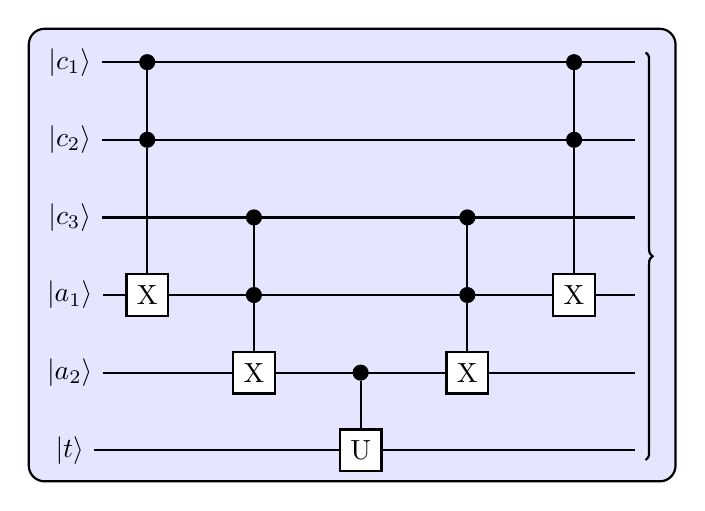
\begin{tikzpicture}[thick]
    % `operator' will only be used by Hadamard (H) gates here.
    % `phase' is used for controlled phase gates (dots).
    % `surround' is used for the background box.
    \tikzstyle{operator} = [draw,fill=white,minimum size=1.5em] 
    \tikzstyle{phase} = [draw,fill,shape=circle,minimum size=5pt,inner sep=0pt]
    \tikzstyle{surround} = [fill=blue!10,thick,draw=black,rounded corners=2mm]
    %
    \matrix[row sep=0.4cm, column sep=0.8cm] (circuit) {
    % First row.
    \node (q1) {\ket{c_1}}; &[-0.5cm] 
    \node[phase] (P11) {} ; & & & &
    \node[phase] (P16) {} ;&[-0.3cm]
    \coordinate (end1); \\
    % Second row.
    \node (q2) {\ket{c_2}}; &
    \node[phase] (P21) {}; & & & & 
    \node[phase] (P26) {} ;&
    \coordinate (end2);\\
    % Third row.
    \node (q3) {\ket{c_3}}; & & 
    \node[phase] (P32) {};  & &
    \node[phase] (P34) {};& 
    & 
    \coordinate (end3); \\
    % Fourth row.
    \node (q4) {\ket{a_1}}; &
    \node[operator] (X41) {X}; &
    \node[phase] (P42) {};  & &
    \node[phase] (P44) {}; &
    \node[operator] (X46) {X}; &
    \coordinate (end4); \\
    % Fifth row.
    \node (q5) {\ket{a_2}}; & &
    \node[operator] (X52) {X};  &
    \node[phase]    (P53) {};&
    \node[operator] (X54) {X};&&
    \coordinate (end5); \\
    % Sixth row.
    \node (q6) {\ket{t}}; & & &
     \node[operator] (U) {U};   & & &;
    \coordinate (end6); \\
    };
    % Draw bracket on right with resultant state.
    \draw[decorate,decoration={brace},thick]
        ($(circuit.north east)-(0cm,0.3cm)$)
        to node[midway,right] (bracket) {}
        ($(circuit.south east)+(0cm,0.3cm)$);
    \begin{pgfonlayer}{background}
        % Draw background box.
        \node[surround] (background) [fit = (q1) (U) (bracket)] {};
        % Draw lines.
        \draw[thick] (q1) -- (end1)  (q2) -- (end2) (q3) -- (end3) (q4) -- (end4) (q5) -- (end5) (q6) -- (end6) (P11) -- (P21) (P21) -- (X41)  (P32) -- (P42) (P42) -- (X52) (P53) -- (U) (P16) -- (P26) (P26) -- (X46) (P34) -- (P44) (P44) -- (X54);
    \end{pgfonlayer}
    %
    \end{tikzpicture}


\subsection{Craig Gidney (we'll name it properly after)}

\begin{itemize}
    \item 2-qubit gates: $8(k-2) + 1$,
    \item 1-qubit gates: $k-2$,
    \item TOTAL gates: $9(k-2)$,
    \item Auxiliary qubits: $k-1$.
\end{itemize}



\section{Conclusion}\label{sec:conclusion}


\bibliography{refs}
\bibliographystyle{plain}
\end{document}